% !TEX TS-program = xelatex
% !TEX encoding = UTF-8

\documentclass[12pt]{article}

\usepackage{fontspec} % Font selection for XeLaTeX; see fontspec.pdf for documentation
\defaultfontfeatures{Mapping=tex-text} % to support TeX conventions like ``---''
\usepackage{xunicode} % Unicode support for LaTeX character names (accents, European chars, etc)
\usepackage{xltxtra} % Extra customizations for XeLaTeX

\usepackage[parfill]{parskip} % Activate to begin paragraphs with an empty line rather than an indent

\usepackage{graphicx} % support the \includegraphics command and options

\usepackage{listings}
\lstset{basicstyle=\ttfamily,columns=fullflexible,keepspaces=true}

%%%%%%%%%%%%%%%%%%%%%%%%%%%%%%%%%%%%%%%%%%%%%%%%%%

\title{Report 3: CUDA}
\author{Dinh Ngoc Tu}

\begin{document}
\maketitle

%%%%%%%%%%%%%%%%%%%%%%%%%%%%%%%%%%%%%%%%%%%%%%%%%%

\section{Implementation}

First, we calculated the dimension of the picture:

\begin{lstlisting}[breaklines]
long long pixelCount = inputImage->width * inputImage->height;
char *blockSizeEnv = getenv("LW3_CUDA_BLOCK_SIZE");
if (!blockSizeEnv) {
    fprintf(stderr, "invalid block size\n");
    return 0;
}
int blockSize = atoi(blockSizeEnv);
long long numBlocks = pixelCount / blockSize + 1;
\end{lstlisting}

We then allocated input and output buffers on the device:
\begin{lstlisting}[breaklines]
uchar3 *inputCudaBuffer;
cudaMalloc(&inputCudaBuffer, pixelCount * sizeof(uchar3));
uchar3 *outputCudaBuffer;
cudaMalloc(&outputCudaBuffer, pixelCount * sizeof(uchar3));
\end{lstlisting}

We copied the source buffer to the on-device buffer, run the code, and retrieve the results:

\begin{lstlisting}[breaklines]
if (cudaMemcpy(inputCudaBuffer, inputImage->buffer, pixelCount * sizeof(uchar3), cudaMemcpyHostToDevice) != cudaSuccess) {
    fprintf(stderr, "input buffer copy error\n");
    return 0;
}
for (int j = 0; j < 100; j++) {
    labwork3<<<numBlocks, blockSize>>>(inputCudaBuffer, outputCudaBuffer, pixelCount);
}
if (cudaMemcpy(outputImage, outputCudaBuffer, pixelCount * sizeof(uchar3), cudaMemcpyDeviceToHost) != cudaSuccess) {
    fprintf(stderr, "output buffer copy error\n");
    return 0;
}
\end{lstlisting}

The CUDA code is implemented as follows:

\begin{lstlisting}[breaklines]
__global__ void labwork3(uchar3 * __restrict__ input, uchar3 * __restrict__ output, long long pixelCount) {
    long long i = threadIdx.x + blockIdx.x * blockDim.x;
    if (i < pixelCount) {
        output[i].x = (char)(((int)input[i].x + input[i].y + input[i].z) / 3);
        output[i].y = output[i].z = output[i].x;
    }
}
\end{lstlisting}

%%%%%%%%%%%%%%%%%%%%%%%%%%%%%%%%%%%%%%%%%%%%%%%%%%

\section{Speedup}

The speedup is as follows:

\begin{figure}[h]
    \caption{Speedup with CUDA}
    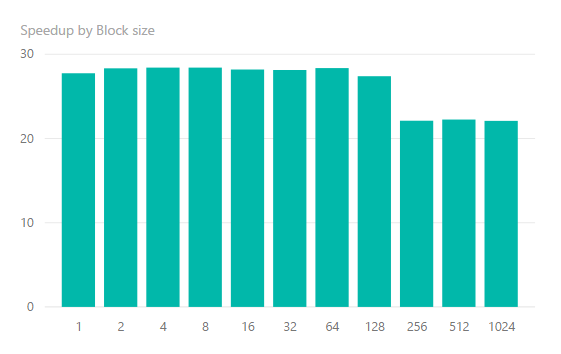
\includegraphics{pics/lw3.png}
\end{figure}

As shown on the graph above, the speedup given by CUDA is anywhere from 22x to 28x depending on block size, and stays quite consistent
between block sizes.
However, block sizes 128 and above are slower than the other block sizes.

%%%%%%%%%%%%%%%%%%%%%%%%%%%%%%%%%%%%%%%%%%%%%%%%%%

\end{document}